\documentclass[12pt, a4paper]{report}
\usepackage{graphicx}
\usepackage{amsmath}
\usepackage{float}
\renewcommand{\baselinestretch}{1.2} 
\usepackage{ragged2e}
\usepackage{fancyvrb}
\usepackage{amssymb}
\usepackage[a4paper, total={7in, 9in}]{geometry}
\usepackage[utf8]{inputenc}
\usepackage{physics}
\usepackage{enumitem}


\title{\textbf{EE2703 : Applied Programming Lab \\ Assignment 9 \\ Discrete Fourier Transform}} % Title
\author{Arun Krishna A M S \\ EE19B001} % Author name
\date{21st May 2021} % Date for the report

\begin{document}		
		
\maketitle % Insert the title, author and date
\justifying

\section*{Introduction}
The \textbf{Discrete Fourier Transform}(DFT) converts a finite sequence of equally-spaced samples of a function into a same-length sequence of equally-spaced samples of the \textbf{discrete-time fourier transform} (DTFT) - a complex-valued function of frequency. Through this assignment, 
\begin{itemize}
  	\item We explore the discrete fourier transform of given functions using the \textbf{Fast fourier transform} algorithm in the \texttt{numpy.fft} module in python. The \textbf{FFT} algorithm runs in $O(nlogn)$ time.
    \item Determine how the window size/time interval affects the DFT of a signal. 
  	\item Finding the window size/time interval for the lowest error in the calculated fourier transform.
\end{itemize}
The discrete Fourier transform transforms a signal sequence of time interval $N$: $x[n]: x[0], x[1], x[2],$ $x[3].....  x[N-1]$ into $X[n]$ given by
\begin{equation}
X[n] = \sum_{k=0}^{N-1} x[k] e^{-2\pi kn/N}
\end{equation}

To find the DFT of a \texttt{function} in the time interval \texttt{[xmin, xmax]} with sampling frequency \texttt{N} is given by the following code:
\begin{verbatim}
x = np.linspace(xmin, xmax, N + 1)[:-1]
w = np.linspace(-np.pi*N/(xmax-xmin), np.pi*N/(xmax-xmin), N + 1)[:-1]
y = function(x)
Y = np.fft.fftshift(np.fft.fft(y))/N    
phase = np.angle(Y)
\end{verbatim}
The frequencies associated with the DFT \texttt{Y} run are from $[-\frac{\pi N}{T_o},\frac{\pi N}{T_o})$ where $T_o$ is the time interval \texttt{xmax - xmin}. 

\section*{DFT of $sin(5t)$}
The frequency components present in the $sin(5t)$ signal are
\begin{equation*}
sin(5t) = -\frac{j}{2}e^{5jt} + \frac{j}{2}e^{-5jt}
\end{equation*}
So it is to be expected that there are two peaks at $5$ and $-5$ frequencies each with amplitude 0.5 and phase $\frac{\pi}{2}$ and $-\frac{\pi}{2}$. The points marked in the phase response with dark blue color are those frequencies that have a significant magnitude $> 10^{-2}$ with the other frequencies having negligible contribution. 
\clearpage
\begin{center}
	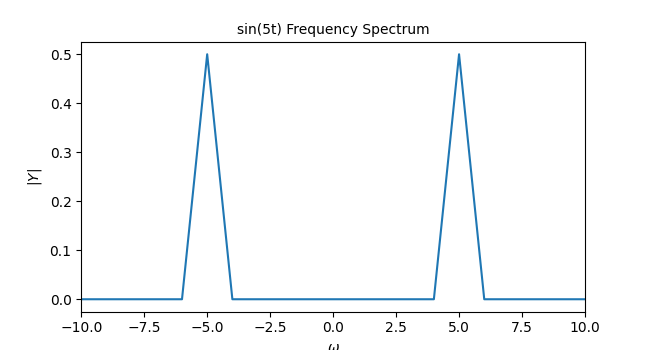
\includegraphics[scale=0.85]{Figure_1.png} 
	\label{fig:rawdata}
\end{center}

\begin{center}
	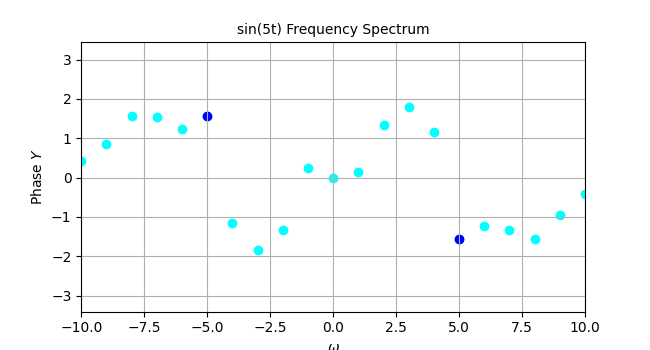
\includegraphics[scale=0.85]{Figure_2.png} 
	\label{fig:rawdata}
\end{center}

\section*{DFT of Amplitude Modulated signal}
Consider the amplitude modulation of $cos(t)$ signal: $(1+ 0.1cos(t))cost(10t)$ with $cos(10t)$ being the carrier frequency. The frequency components associated with this signal are 
\begin{equation*}
(1+ 0.1cos(t))cost(10t) = (1 + \frac{0.1}{2}e^{jt} + \frac{0.1}{2}e^{-jt})(\frac{1}{2}e^{10jt} + \frac{1}{2}e^{-10jt})
\end{equation*}
\begin{equation*}
 = \frac{0.1}{4}e^{9jt} + \frac{0.1}{4}e^{-9jt} + \frac{0.1}{4}e^{11jt} + \frac{0.1}{4}e^{-11jt} + \frac{1}{2}e^{10jt} + \frac{1}{2}e^{-10jt}
\end{equation*}

Thus we can observe the following frequency components: 
\clearpage
\begin{center}
\begin{tabular}{ |c|c| } 
 \hline
frequency & amplitude \\ 
9 & 0.025\\
-9 & 0.025\\
10 & 0.5\\
-10 & 0.5\\
11 & 0.025\\
-11 & 0.025\\
 \hline
\end{tabular}
\end{center}


\begin{center}
	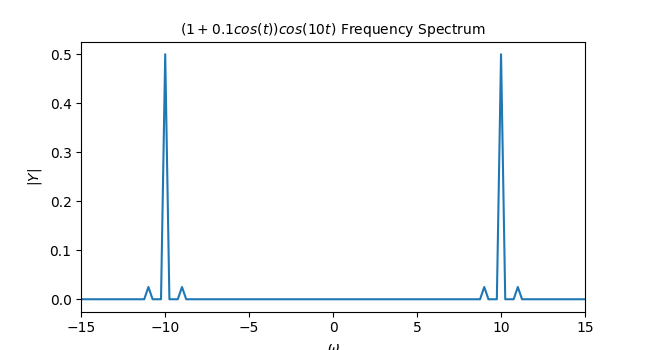
\includegraphics[scale=0.72]{Figure_3.png} 
	\label{fig:rawdata}
\end{center}

\begin{center}
	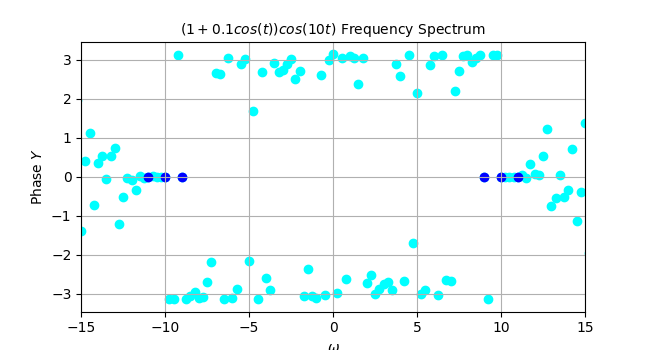
\includegraphics[scale=0.72]{Figure_4.png} 
	\label{fig:rawdata}
\end{center}

\section*{DFT of $sin^3(t)$ and $cos^3(t)$}
Expressing the given functions in terms of sinusoidal harmonics:

\begin{equation*}
sin^3(t) = \frac{3}{4}sin(t) - \frac{1}{4}sin(3t)
\end{equation*}
\begin{equation*}
sin^3(t) = \frac{3j}{8}e^{-jt} - \frac{3j}{8}e^{jt} - \frac{1j}{8}e^{-3jt} + \frac{1j}{8}e^{3jt}
\end{equation*}
\clearpage
\begin{center}
	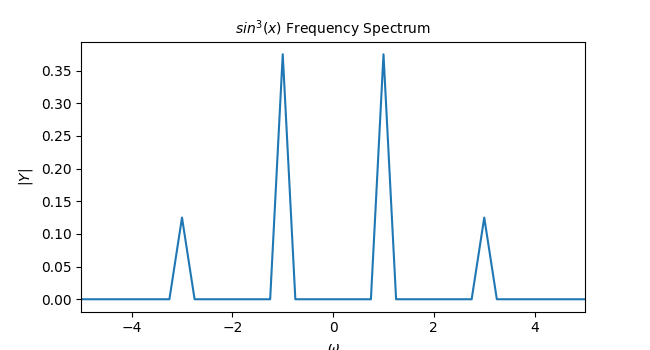
\includegraphics[scale=0.72]{Figure_5.png} 
	\label{fig:rawdata}
\end{center}

\begin{center}
	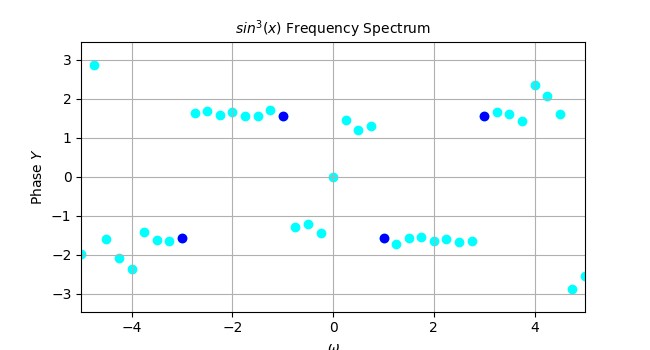
\includegraphics[scale=0.72]{Figure_6.png} 
	\label{fig:rawdata}
\end{center}

\begin{equation*}
cos^3(t) = \frac{1}{4}cos(t) + \frac{3}{4}cos(3t)
\end{equation*}
\begin{equation*}
cos^3(t) = \frac{1}{8}e^{jt} + \frac{1}{8}e^{-jt} + \frac{3}{8}e^{3jt} + \frac{3}{8}e^{-3jt}
\end{equation*}

\begin{center}
	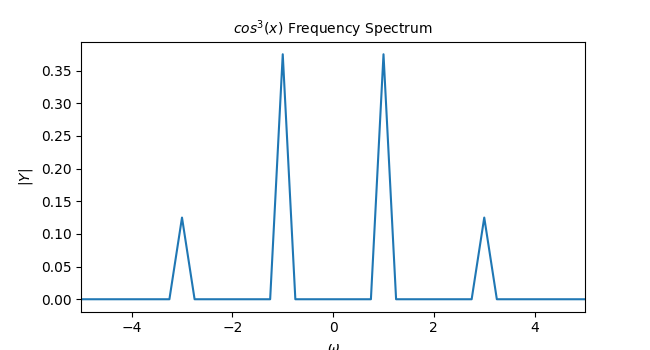
\includegraphics[scale=0.72]{Figure_7.png} 
	\label{fig:rawdata}
\end{center}
\clearpage
\begin{center}
	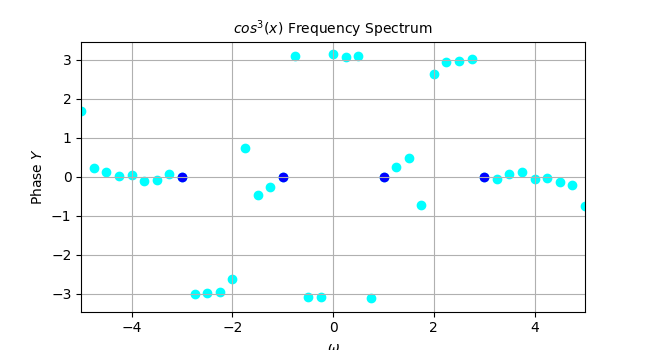
\includegraphics[scale=0.8]{Figure_8.png} 
	\label{fig:rawdata}
\end{center}

\section*{DFT of Phase Modulated signal}
Consider the phase modulation of $cos(t)$ signal: $cos(20t + 5cos(t))$ with $cos(20t)$ being the carrier frequency. To get the frequency spectrum, we can expand the function using \textbf{Jacobi Anger Expansion} which states
\begin{equation}
e^{jzcos(\theta)} = \sum^{\infty}_{n = - \infty} j^n J_n(z)e^{jn\theta}
\end{equation}
where $J_k$ is the $k^{th}$ order \textbf{Bessel Function}. 

Applying this expansion to the signal $cos(\omega_ct + hcos(\omega_mt))$ 
\begin{equation*}
e^{j(\omega_ct + hcos(\omega_mt)} = e^{j\omega_ct}e^{jhcos(\omega_mt)} 
\end{equation*}
\begin{equation*}
e^{j(\omega_ct + hcos(\omega_mt)} = e^{j\omega_ct}\sum_{n = -\infty}^{\infty}J_n(h)e^{jn\omega_mt}j^n = \sum_{n = -\infty}^{\infty}J_n(h)e^{j(\omega_ct + n(\omega_mt + \frac{\pi}{2}))}
\end{equation*}
Taking the real part we arrive at 
\begin{equation}
cos(\omega_ct + hcos(\omega_mt)) = \sum_{n = -\infty}^{\infty}J_n(h)cos(\omega_ct + n(\omega_mt + \frac{\pi}{2}))
\end{equation}
\begin{equation*}
cos(20t + 5cos(t)) = \sum_{n = -\infty}^{\infty}J_n(5)cos(20t + n(5t + \frac{\pi}{2}))
\end{equation*}
This shows us that the bands are centred around $20$ and the amplitude of each frequency component is given by the value of the Bessel function.
\clearpage
\begin{center}
	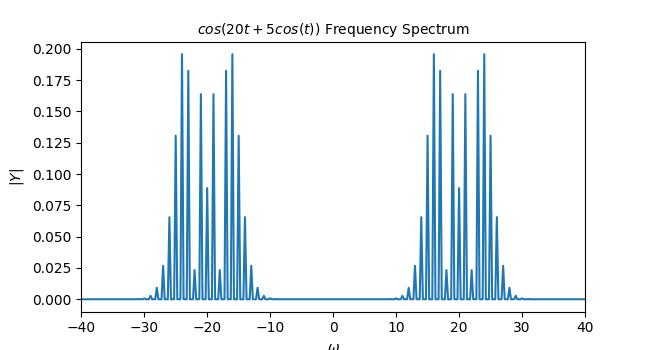
\includegraphics[scale=0.72]{Figure_9.png} 
	\label{fig:rawdata}
\end{center}

\begin{center}
	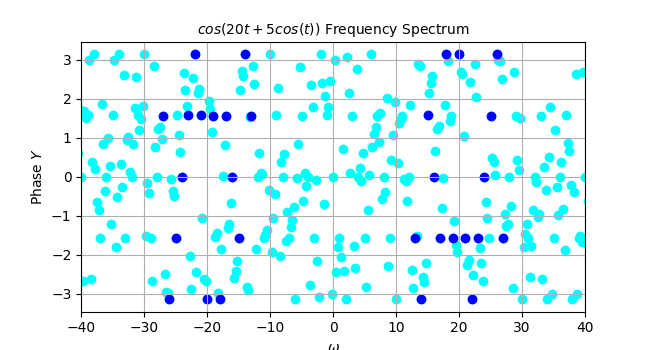
\includegraphics[scale=0.72]{Figure_10.png} 
	\label{fig:rawdata}
\end{center}

\section*{DFT of Gaussian Distribution}
We now analyze the DFT of the Gaussian distribution $e^{\frac{-t^2}{2}}$. It can be observed that the function is non-periodic, i.e., not band-limited - the frequency spectrum can have non-zero values for higher frequencies.
\\
The Continuous Time Fourier Transform of the Gaussian distribution is given by 
\begin{equation*}
\mathcal{F}\{e^{\frac{-t^2}{2}}\} = \sqrt{2\pi}e^{\frac{-\omega^2}{2}}
\end{equation*}
Since the DFT does not exist for a non-periodic function, the function is assumed to be periodic about the chosen interval. As we then increase the time interval, the DFT will approach the Fourier Transform, because at large time periods, the function can be considered approximately aperiodic.

We compare the calculated DFT and the expected DFT for different time intervals, from $[-\pi,\pi)$ to $[-6\pi,6\pi)$ and plot the maximum-error between the expected and calculated. We observe that
\clearpage
\begin{center}
	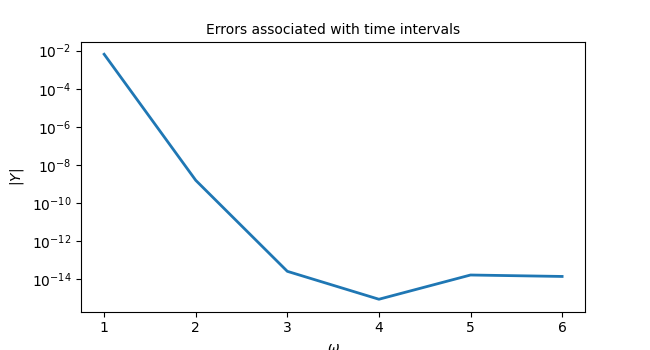
\includegraphics[scale=0.9]{Figure_11.png} 
	\label{fig:rawdata}
\end{center}

\begin{verbatim}
time interval: [-1pi, 1pi) Error = 0.006496802750855624
time interval: [-2pi, 2pi) Error = 1.5607475312151564e-09
time interval: [-3pi, 3pi) Error = 2.5979218776228663e-14
time interval: [-4pi, 4pi) Error = 8.881784197001252e-16
time interval: [-5pi, 5pi) Error = 1.6653345369377348e-14
time interval: [-6pi, 6pi) Error = 1.3988810110276972e-14
\end{verbatim}

As expected the error decreases rapidly with increase in the window size. The expected plot is a Gaussian function with the phase being zero since it is real valued.

\begin{center}
	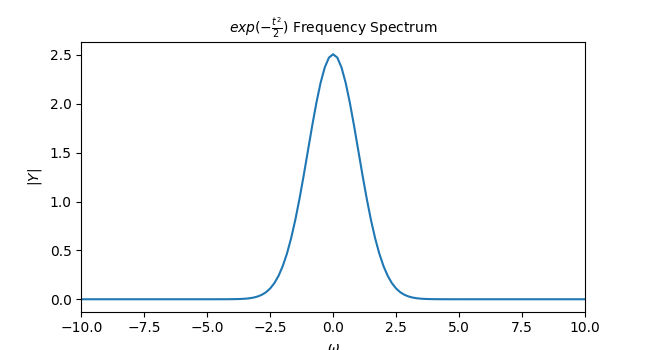
\includegraphics[scale=0.8]{Figure_12.png} 
	\label{fig:rawdata}
\end{center}
\clearpage
\begin{center}
	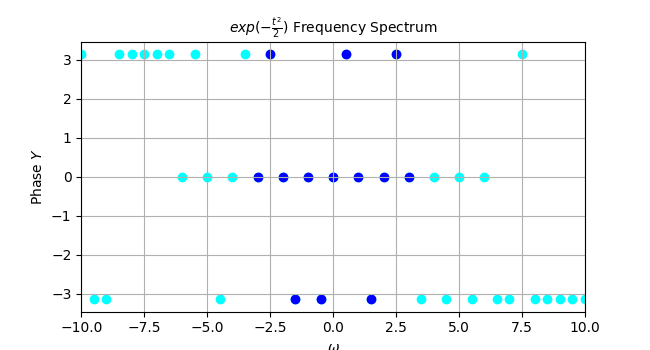
\includegraphics[scale=0.8]{Figure_13.png} 
	\label{fig:rawdata}
\end{center}

\section*{Conclusion}
Using the \texttt{numpy.fft} module, the discrete fourier transform of various signals: sinusoids, AM, PM & Gauss distribution were evaluated and plotted. We also observed how \textbf{Bessel Functions} were used to calculate the DFT for a phase modulated signal. We also observed how an increase in the time period, reduces the error of DFT of an aperiodic signal.
\end{document}

